\chapter{Quality control in orientation}

This chapter covers different aspect of quality control of orientation.


    % - - - - - - - - - - - - - - - - - - - - - - - - - - - - - - - -
    % - - - - - - - - - - - - - - - - - - - - - - - - - - - - - - - -
    % - - - - - - - - - - - - - - - - - - - - - - - - - - - - - - - -

\section{Sensibility Analysis : Theoreticall consideration}

\subsection{some tricks}

\subsubsection{tricks}
When $A$ and $B$ are vector, $ \transs A  B$ is as scalar so :


\begin{equation}
     \transs A B =  \transs ( \transs A B) =  \transss B A  \label{Trick:tABEqtBA}
\end{equation}

Then  :

\begin{equation}
     (^t A  B) ^2 =  ^t A B ^t B A  = ^t A (B ^t B) A \label{Trick:tAB2}
\end{equation}

So the term can interpred as the application of the quadratic form $B ^t B$  \footnote{of rank $1$}  to vector $A$.

\subsubsection{tricks}

If $A$ is a symetric positive matrix,
the minimum of quadratic form $F(X) = ^t X A X - 2^t B X$ is reached for $X=A^{-1} B$.
If we write $X' = X + \delta $ :

\begin{equation}
  F(X') -F(X)  = ^t (A^{-1} B+\delta) A (A^{-1} B+\delta) -  2^t B (A^{-1} B + \delta) -F(X)
          =  ^t \delta A \delta 
\end{equation}

Which is always positive as $A$ is positive.

\subsubsection{tricks}
We have also the well known block matrix inverse identity :

\begin{equation}
\left( \begin{array}{cc} 
              A & B \\ 
              C  & D\\ 
        \end{array} 
\right) ^{-1}
= 
\left( \begin{array}{cc} 
              A' & B' \\ 
              C'  & D'\\ 
        \end{array} 
\right) 
= 
\left( \begin{array}{cc} 
              (A-BD^{-1}C)^{-1} & -(A-BD^{-1}C)^{-1} BD^{-1} \\ 
              -D^{-1}C(A-BD^{-1}C)^{-1}  &  D^{-1}+D^{-1}C(A-BD^{-1}C) BD^{-1}\\ 
        \end{array} 
\right) 
\label{Eq:BlockInv}
\end{equation}


    % - - - - - - - - - - - - - - - - - - - - - - - - - - - - - - - -
    % - - - - - - - - - - - - - - - - - - - - - - - - - - - - - - - -
    % - - - - - - - - - - - - - - - - - - - - - - - - - - - - - - - -


\subsection{Least square notation}

Suppose we have $M$ equation of observation with $N$ unknown, $M>N$ :

\begin{equation}
    \sum\limits_{i=1}^N l_i^ m x_i = o_m \; ; \label{Eq:LeastSq:1}
\end{equation}

Noting :
\begin{equation}
    L^m = ^t (l_1^m \;  l_2^m \dots l_N^m)  m \in [1,M] ;  X= ^t (x_1 \; x_2 \dots x_N) 
\end{equation}

Equation~\ref{Eq:LeastSq:1} writes :

\begin{equation}
     ^t L^m  X  = o_m \; ,  m \in [1,M] ;
\end{equation}


As $M>N$ it is generally impossible to annulate all the term , instead we minimise the square of residual $R_2(X)$  :

\begin{equation}
    R^2(X) = \sum\limits_{m=1}^M ( ^tL^m   X - o_m) ^2  
\end{equation}

Using tricks \ref{Trick:tABEqtBA} and \ref{Trick:tAB2} we can write :

\begin{equation}
    R^2(X) = \sum\limits_{m=1}^M  ( (^tL^m   X)^2 - 2 o_m {^tL^m} X + o_m ^ 2) 
           = \sum\limits_{m=1}^M  ( {^t X ({L^m} ^t{L^m}) X} - (2 o_m {^tL^m} )X + o_m ^2)
\end{equation}


Noting the $N \times N$ matrix A, $B$ the $N$ vector and the scalar C :

\begin{equation}
           A = \sum\limits_{m=1}^M { ({L^m} ^t{L^m}) } 
       ;\; B = \sum\limits_{m=1}^M  ( o_m {L^m} ) 
       ;\; C = \sum\limits_{m=1}^M  o_m ^2
 \label{LeastSq:ABC}
\end{equation}

We have :

\begin{equation}
    R^2(X) = ^t X A X - 2^t B X + C
\end{equation}

Obviously $A$ is positive as being the some of squares. The minimum is reached for :

\begin{equation}
     \hat{X}  =  A^{-1} B
\end{equation}

%------------------------ Variance ------------------------------------------

\subsection{Variance}
\label{Sec:VarLsq}

The system being not exactly invertible, for each observation $m$,  
the equation~\ref{Eq:LeastSq:1} is only approximatively satisified by $\hat{X}$,
so we introduce the  residual $\epsilon$  to modelize this uncertainty:

\begin{equation}
     ^tL^m X = o_m + {\epsilon}_m
\end{equation}

To evaluate variance on $X$ we consider  ${\epsilon}_m$  as the realization of random variable. Here I consider that 
each ${\epsilon}_m$ is an indepandant variable, of average $0$ and variance $r_m^2$ \footnote{well  it's probably an heresy
for stasticall point of view to try ro extract information from a single realisation ?} where $r_m^2$ is the empirical residual :


\begin{equation}
      r_m  = ^tL^m \hat{X} - o_m  ; Var({\epsilon}_m) = r_m^2
      \label{Eq:Empir:Var}
\end{equation}

We can then modelize the probabilistic aspect of evaluation of $X$ by the random vector $\tilde X$ :

\begin{equation}
     \tilde X  =  A^{-1}  \sum\limits_{i=1}^M   {L^m}  (o_m + {\epsilon}_m) 
\end{equation}

As $o_m$ is deterministic the variance is :

\begin{equation}
     Var(\tilde X)  =  Var (A^{-1}  \sum\limits_{i=1}^M   {L^m}  {\epsilon}_m)
\end{equation}


Noting the element of $A^{-1}$ :

\begin{equation}
     A^{-1} = ( {a'}_i^j)
\end{equation}

\begin{equation}
     Var( \tilde x_i)  =   Var({\sum\limits_{m=1}^M}  {\sum\limits_{j=1}^N}  {a'}_i^j   {l^m_j}   {\epsilon}_m)
\end{equation}


\begin{equation}
     Var( \tilde x_i)  =   \sum\limits_{m=1}^M  Var({\epsilon}_m)  (\sum\limits_{j=1}^N   {a'}_i^j  {l^m_j}   ) ^2 
\end{equation}



\begin{equation}
     Var(\tilde x_i) = \sum\limits_{m=1}^M (^tL^m \hat{X} - o_m )^2 (\sum\limits_{j=1}^N {a'}_i^j {l^m_j})^2 
\end{equation}

%------------------------ Co-Variance ------------------------------------------

\subsection{Covariance}
\label{Sec:CovLsq}

Similarly, we can compute the covariance :

\begin{equation}
     Cov(\tilde x_i \tilde x_j)  =   \mathbb{E} (
                            ({\sum\limits_{m=1}^M}  {\sum\limits_{k=1}^N}  {a'}_i^k   {l^m_k}   {\epsilon}_m)
                            ({\sum\limits_{n=1}^M}  {\sum\limits_{k=1}^n}  {a'}_i^k   {l^n_k}   {\epsilon}_n)
                       )
\end{equation}

Under the independance hyopthesis, we have


\begin{equation} 
  \forall m,n ,  m\neq n : \mathbb{E} ({\epsilon}_m {\epsilon}_n) = 0 
\end{equation}


\begin{equation}
     Cov(\tilde x_i \tilde x_j)  =     \sum\limits_{m=1}^M  Var({\epsilon}_m) 
                         (\sum\limits_{k=1}^N  {a'}^k_j   {l^m_k}  )
                         (\sum\limits_{k=1}^N  {a'}^k_i   {l^m_k}  )
\end{equation}


%------------------------ Unown substitution ------------------------------------------

\subsection{Unknown elimination}

Computation of variance and co-variance  requires some additional precaution when using
the schurr complement technique as  described in~\ref{UnkAux:Algeb} and~\ref{UnkAux:Var}.
The computation of this paragraph are rather destinated to understant the code modification
impacted by unkown elimination.


We separate the unkown in $X$ and $Y$, where $X$ is the unknown we want to eliminate.

\begin{equation}
     \transK ^m X +  \transL ^m Y  = o_m 
\end{equation}

And the residual  writes : 

\begin{equation}
      R^2 (X,Y) =  \transX (\sum\limits_{m=1}^M  K^m {\transKm} ) X    
                  + 2 (\sum\limits_{m=1}^M  (\transLm Y - o_m  )  \transKm ) X
                  +   \sum\limits_{m=1}^M  (\transLm Y - o_m  ) ^2
\end{equation}

We split $R^2$  in $R^2_y(Y)$ and $r_Y(X)$, where  $R^2_y$ is the part that do not depends of $X$   : 

\begin{equation}
       \Lambda = \sum\limits_{m=1}^M  \KmtKm                       \;\;\;  ; \;
       \Gamma(Y)  = \sum\limits_{m=1}^M  (\transLm Y - o_m  ) K^m 
\end{equation}
\begin{equation}
       r_Y (X) =  ^tX  \Lambda  X    + 2   ^t \Gamma(Y)  X   \;\;\;  ; \;
       R_y^2 (Y) =  \sum\limits_{m=1}^M  (\transLm Y - o_m  ) ^2 
\end{equation}

\begin{equation}
      R^2 (X,Y) =   r_Y(X) +    R_y^2 (Y)  
\end{equation}



To eliminate $X$ in the minimisation, we set $X$  to the value that minimize $r_Y(X)$ for a given  $Y$,
that is :

\begin{equation}
    \hat{X}(Y) = -  \Lambda^{-1}  \Gamma(Y)
    \label{Eq:XHatOfY}
\end{equation}

And the minimum value is :

\begin{equation}
    r_Y(\hat{X}(Y)) 
    = ^t\hat{X}(Y)  \Lambda  \hat{X}(Y)    + 2   ^t \Gamma(Y)  \hat{X}(Y) 
   =   - ^t \Gamma(Y) \Lambda^{-1} \Gamma(Y)
\end{equation}


In unkown elimination we suppose that $X=\hat{X}(Y)$ and compute only : 

\begin{equation}
      \breve{R}^2 (Y) = R^2(\hat{X}(Y),Y)  =     R_y^2 (Y)   -  ^t \Gamma(Y) \Lambda^{-1} \Gamma(Y)
\end{equation}

We develop :

\begin{equation}    \breve{R}^2 (Y) =
                       \sum\limits_{m=1}^M  (\trans L^m Y - o_m  ) ^2
                  -    (\sum\limits_{m=1}^M  (\trans L^m Y - o_m  )  \trans K^m )  
                       \Lambda^{-1}
                       (\sum\limits_{m=1}^M  (\trans L^m Y - o_m  )  K^m ) 
\end{equation}

Noting :


\begin{equation}  
     \breve{A} =  \sum\limits_{m=1}^M{L^m}{\trans L^m}
               -(\sum\limits_{m=1}^M {L^m} \trans {K^m})   \Lambda^{-1}  (\sum\limits_{m=1}^M   {K^m} \trans {L^m} ) 
\end{equation}  

\begin{equation}  
     \breve{B}  =   \sum\limits_{m=1}^M (o_m L^m ) 
                - (\sum\limits_{m=1}^M  {L^m}  \trans K^m) \Lambda^{-1}  (\sum\limits_{m=1}^M o_m K^m )
\label{Var:BChap}
\end{equation}  

We have :

\begin{equation}  
      \breve{R}^2 (Y) = \trans Y \breve{A} Y - 2  \trans \breve{B}  Y + Cste
\end{equation}


And the estimation of $\breve{Y}$ of $Y$ by least square : 


\begin{equation}  
      \breve{Y} =  \breve{A}^{-1}  \breve{B}
\end{equation}

We write :

\begin{equation}  
     \Theta =  \sum\limits_{m=1}^M {L^m} \trans {K^m}   
\end{equation}  


\begin{equation}  
     \breve{A} =  \sum\limits_{m=1}^M{L^m}{\trans {L^m}} - \Theta \Lambda^{-1}   {\trans} \Theta 
     \label{FinalBreveA}
\end{equation}  

\begin{equation}  
     \breve{B}  =   \sum\limits_{m=1}^M (o_m L^m ) 
                - \Theta \Lambda^{-1}  (\sum\limits_{m=1}^M o_m K^m )
               = \sum\limits_{m=1}^M  o_m (L^m -\Theta \Lambda^{-1} K^m)
     \label{FinalBreveB}
\end{equation}  

Defining $\breve{L}^m$, we have :

\begin{equation}  
     \breve{L}^m   =   (L^m  - \Theta  \Lambda^{-1} K^m)
\end{equation}  

\begin{equation}  
     \breve{B}  = \sum\limits_{m=1}^M  o_m \breve{L}^m
\end{equation}  


Using $\breve{A}$, $\breve{B}$  and $\breve{L}^m$ we finaly can compute the variance and
covariance of $\breve Y$ with formula equivalent to~\ref{Sec:VarLsq} and~\ref{Sec:CovLsq}~.
We consider the random vector $\tilde Y$ :

\begin{equation}  
     \tilde{Y}  =   \breve{A}^{-1}  \sum\limits_{m=1}^M  (o_m + \epsilon _m) \breve{L}^m
\end{equation}  

We have :

\begin{equation}
     Var(\tilde{y}_i) =  \sum\limits_{m=1}^M  Var(\epsilon _m)  (\sum\limits_{j=1}^N {\breve {a}'}{_i^j}  {\breve l}{^m_j})^2 
\label{Final:Var}
\end{equation}


\begin{equation}
     Cov(\tilde y_i \tilde y_j)  =     \sum\limits_{m=1}^M  Var({\epsilon}_m) 
                         (\sum\limits_{k=1}^N  {\breve {a'}}^k_j   {\breve {l}}^m_k  )
                         (\sum\limits_{k=1}^N  {\breve {a'}}^k_i   {\breve {l}}^m_k  )
\end{equation}

\subsection{Practicle aspects on unknown elimination in MicMac}

Practically, in MicMac, the unkwon elimination is essentially used  to eliminate, for each tie points, 
the $3$d point that project on each image. This is done "\`a la vol\'ee" (on the flight ?) with
the following procedure, for each tie point :

\begin{itemize}
    \item the unknown of the $3d$ point are always located to the same place (say they are unknown $1,2,3$)
    \item the observation are used in accumulator matrix $A,B,C$ using equation \ref{LeastSq:ABC} (ignoring
          for now the future elimination);
    \item  then $\Lambda$ and $\Theta$ are computed and equations \ref{FinalBreveA} and \ref{FinalBreveB} to
           modify the accumulator $A,B,C$
    \item the part of the accumulator $A,B,C$  corresponding to unknow $[1-3]$ are reseted;
\end{itemize}

So at the end, the accumulator $A$ and $B$ contains the  global $\breve A$  and $\breve B$ and allow to
compute the optimal value $\breve Y$ . For variance-covariance,
this way of proceeding ,  raise a probleme for computing the residual for estimation of $Var(\epsilon _m)$  that
require the value of unknowns as shown in \ref{Eq:Empir:Var}, we know the value for $Y$, but not for $X$.
There is two possibility :

\begin{itemize}
   \item  use  formula \ref{Eq:XHatOfY} , with  $\breve Y$  as value, this create an iteration offset;
   \item use the value computed from bundle intersection, which is also an approximation.
\end{itemize}

For now the second solution is used .



    % - - - - - - - - - - - - - - - - - - - - - - - - - - - - - - - -
    % - - - - - - - - - - - - - - - - - - - - - - - - - - - - - - - -
    % - - - - - - - - - - - - - - - - - - - - - - - - - - - - - - - -

\subsection{Sensibility}


\begin{equation}
F(X) = ^t X M X = F(y,Z)= 
\left( \begin{array}{cc} 
              y &  ^t Z \\ 
        \end{array} 
\right)
\left( \begin{array}{cc} 
              a & B \\ 
              ^t B  & D\\ 
        \end{array} 
\right)
\left( \begin{array}{c} 
              y \\ 
              Z \\ 
        \end{array} 
\right)
= a y^2 + 2y^t B Z + ^t Z D Z
\label{EqSensib1}
\end{equation}

For a given $y$, $F(y,Z)$ is minimal for :

\begin{equation}
Z_{min}(y) = -y  D^{-1} B
\end{equation}

And the minimal value is :

\begin{equation}
V_{min}(y) = F(y,Z_{min}(y)) =  y^2 (a- ^t B D^{-1} B)
\end{equation}


In our  case where $A=a$ is a $1$ dimensionnal (scalar) we can then write :

\begin{equation}
V_{min}(y) =   y^2 (a- ^t B D^{-1} B) = \frac{x^2}{a'}
\end{equation}

So using equation ~\ref{Eq:BlockInv}, $V_{min}(x)$ can be easily computed  from the inverse matric. If
we have a "bad" value of $y$, we have two estimation of the impact
on  $F$ :

\begin{itemize}
   \item a "pessimistic" $a y^2$;
   \item a "optimistic" $\frac{y^2}{a'}$.
\end{itemize}

So know, if we explain the empirical least square error $R$, by
a bad estimation on $y$, we have two estimation of the sensibility/accuracy of $y$ ,
optimisitic in \ref{Sens:Optim} and pessimistic in \ref{Pess}:

\begin{equation}
  \sqrt{\frac{a}{R}}
  \label{Sens:Optim}
\end{equation}


\begin{equation}
  \sqrt{a'R}
  \label{Sens:Pess}
\end{equation}

    % - - - - - - - - - - - - - - - - - - - - - - - - - - - - - - - -
    % - - - - - - - - - - - - - - - - - - - - - - - - - - - - - - - -
    % - - - - - - - - - - - - - - - - - - - - - - - - - - - - - - - -

\section{Structureless merging by covariance propagation}

\subsection{Motivation and notation}

The aim this section is to describe a methodology for integrating
result of relative orientation into a global orientation.

We note  $I_k, k \in [1,N] $ the images.
We note  $P_k = (R_k , C_k) $ the pose of image $I_k$ we want to estimate.
With $R_k$ the rotation and $C_k$ the center.

By some language abuse we identify the $P_k$ and the $\mathbb{R}^3 \to  \mathbb{R}^3$ maping
that transformate camera coordinates into word coordinates :

\begin{equation}
   P_k(q) = C_k + R_k q
\end{equation}


\begin{equation}
\begin{tikzcd}
   W_k \arrow[r, "P_k"] &  \omega
\end{tikzcd}
\end{equation}

With this assimilation, we have the standard composition law :

\begin{equation}
   P_1 P_2 = (C_1 + R_1 C_2, R_1 R_2)
\end{equation}

We suppose we have computed relative orientation for a number of subset
of images. Theses subset can be pair, triplet, $N$-uplet, this does
not matter in the formalism.  In many approach authors restrict to
pairs, in our approach we use pair and triplets, but there is
no theoreticall restriction to use quadruplet, quintuplet ...  This is
a practicle aspect of how to select a manageable number of subset,  who leads in
general to select only pairs, or pairs and triplets.


In structureless we have a set of  $M$ subsets  $E^i, \; i \in [1,M]$, 
we note   $E^i =  \{I_{k^i_j}\}$ with $j \in [1,n_i]$  .  For each $E_i$
we have computed a relative orientation of each subset.  We note $p^i_j = (c^i_j,r^i_j)$ the pose
estimated for image $I_{k^i_j}$     in subset $E^i$. 

If the computation of $P_k$ and $p^i_j$  were errorless, there would
exist a $3d$ similitude $\mathcal{S}^i = (\lambda^i ,\mathcal {R}^i ,\mathcal{C}^i) $ for each subset such as :


\begin{equation}
\begin{tikzcd}
     W_{k^j} \arrow[rd,"p^i_j"]\arrow[r, "P_{k^i_j}"] & \omega   \arrow[d, "S_i" ]   \\
                                  & \omega_i
\end{tikzcd}
\end{equation}

\begin{equation}
    \mathcal{S}^i  P_k   =   (\mathcal{C}^i + \lambda^i C_k, \mathcal{R}^i  R_k ) \label{Eq:Def:Sim}
\end{equation}

\begin{equation}
    \mathcal{S}^i  P_{k^i_j}  =  p^i_j  ,\,  \forall i \in [1,M] , \, j \in [1,n_i] \label{Eq:Cov:Sim}
\end{equation}


Structurelless bunble adjustment can be formulated as the problem of computing,
up to a global similitude, the $P_k$ from the $p^i_j$ using equation~\ref{Eq:Cov:Sim}.
Most of the existing approach use a fixed  metric $||\;||$ on poses, an try to compute  solution
minimizing some function like :

\begin{equation}
    \sum\limits_{\substack{i=1 }}^{M} \sum \limits_{\substack{j=1 }}^{n_i}  || \mathcal{S}^i  P_{k^i_j} , p^i_j  ||  \label{Eq:Cov:MinDist}
\end{equation}

Also this approach may be suitable to compute an initial solution, it can
be sometime very unacurate.  Because, using a unique metrics, it doesnt take
into account that, depending on the configuration, there exist parameters
than can be estimate very unacurately in the $E^i$. 

This is illustrated, on figures~\ref{Fig:Cov:Overlap} and~\ref{Fig:Cov:TwoSol}, 
with the realistic example which would be typicall from 
an aerial acquisition  :

\begin{itemize}
    \item  lelft figure~\ref{Fig:Cov:Overlap} represents a typical overlap of
          a so called $60\% \times 20\%$ flight acquisition;
    \item  right figure~\ref{Fig:Cov:Overlap} zoom on image $I_{11}$ and $I_{21}$
          overlap.
\end{itemize}



\begin{figure}
\begin{center}
\begin{tabular}{||c|c||}
   \hline \hline
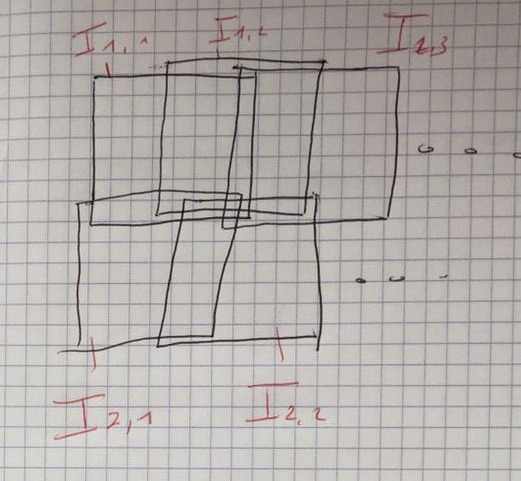
\includegraphics[width=70mm]{FIGS/Cov/Global.jpeg} &
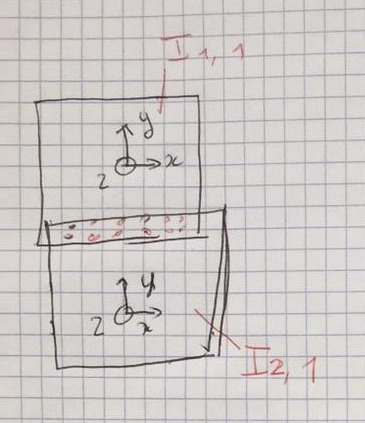
\includegraphics[width=50mm]{FIGS/Cov/TwoIm.jpeg} \\
  \\ \hline  \hline
\end{tabular}
\label{Fig:Cov:Overlap}
\caption{A global view of overlapping image and a zoom on $I_{11}$ and $I_21$}
\end{center}
\end{figure}


\begin{figure}
\begin{center}
\begin{tabular}{||c|c||}
   \hline \hline
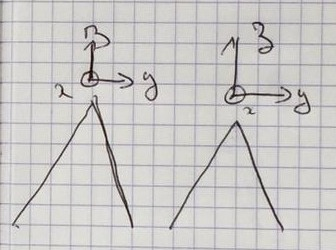
\includegraphics[width=50mm]{FIGS/Cov/Sol1.jpeg} &
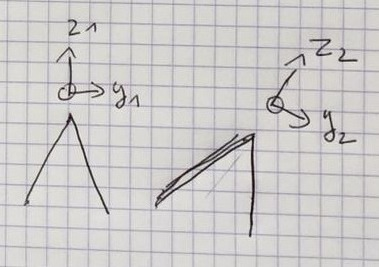
\includegraphics[width=50mm]{FIGS/Cov/Sol2.jpeg} \\
  \\ \hline  \hline
\end{tabular}
\label{Fig:Cov:TwoSol}
\caption{Two likely solution to relative orientation of $I_{11}$ and $I_21$}
\end{center}
\end{figure}



It is well known that in such configuration,  there is a high correlation between
translation in $Oy$ and rotation arround $Ox$. This correlation is specially high
with long focal and flat terrain. In such configuration the two solution of figure
\ref{Fig:Cov:TwoSol} are likely two occurs when computing relative orientation of $I_{11}$ and $I_{21}$.


Suppose for exemple that left configuration is the real one, but that computation return the
right one.  So if we inject this solution in  minimization of formula \ref{Eq:Cov:MinDist} we 
will force  orientation to a false value. Maybe it will be partially eliminated by some 
robust criterion in implementation of \ref{Eq:Cov:MinDist}, but obviously there is a risk
to have some bias if the inlier in relative solutions are not dominating.

However, we are not obliged to create this false information and to treat equally variable
that are accurately estimated and variable that are unaccurately estimated. If we have
the variance/covariance matrix resulting from relative orientation, we can use it to
to inject exactly what we know, and no more, in equation~\ref{Eq:Cov:MinDist}.

In fact, when soluton $p^i_j$  result from a local bundle adjsutment on $E^i$,
we have computed this covariance and can use it.
This is the purpose of the method we desribe now.


    % - - - - - - - - - - - - - - - - - - - - - - - - - - - - - - - -
    % - - - - - - - - - - - - - - - - - - - - - - - - - - - - - - - -
    % - - - - - - - - - - - - - - - - - - - - - - - - - - - - - - - -

\subsection{Hypothesis and aims}

In this part of the description, the proposed method make the following assumption :

\begin{itemize}
   \item $H1$ we have already computed the \emph{precise} relative orientation $p^i_j$  for all $E^i$;
   \item $H2$ we have already computed an \emph{approximate} solution to gobal orientation $P'_k$.
\end{itemize}

The aim of the method is to compute a more precise $P_k$ using  $p^i_j$  and $P'_k$, with
fast computation not requiring to use all tie-points in a global bundle.

Obviously, hypothesis $H2$ may seems too restrictive as having a not too bad global solution 
is a hard point.  It could  even be argued that we propose a complex method for solving
the easy part supposing the most complicated stuff has already been resolved \dots   In fact,
this is not the case :

\begin{itemize}
   \item robust methods for computing  global solution, are generally iterative or hierarchical;
   \item in both case they begin with small subset, for which the global solution is easy to compute;
   \item they use iteration during wich  they make grow the subsets , 
   \item at each iteration, they compute a initial solution for the additional pose and need to
         do some work to reduce propagation error;
\end{itemize}

So in fact, the method proposed must rather be thought as an element of a global initialization
where it is used at the step of refinement of current solutions. By the way, to keep it simple,
we will adopt $H1$ and $H2$.


    % - - - - - - - - - - - - - - - - - - - - - - - - - - - - - - - -
    % - - - - - - - - - - - - - - - - - - - - - - - - - - - - - - - -
    % - - - - - - - - - - - - - - - - - - - - - - - - - - - - - - - -

\subsection{Structureless covariance , case known similitude}

We begin by an approximate but simpler process. The process is $5$ steps :

\begin{enumerate}
    \item compute the  $p^i_j$ in each $E^i$  (it is $H1$);
    \item compute the  covariance matrix $a^i$ and  vector $b^i$  in each $E^i$;
    \item estimate similitude $\mathcal{S}^i$  ;
    \item use $\mathcal{S}^i$ to transfer local $a^i,b^i$ to global $A_i,B_i$ and accumulate  
          $A_i$ and $B_i$ in a global system $A$ and $B$
    \item use $A$ and $B$ to refine the global solution.
\end{enumerate}

    % - - - - - - - - - - - - - - - - - - - - - - - - - - - - - - - -

\subsubsection{compute accurate  $p^i_j$ }

We can use the approach use in {\tt Martini} :

\begin{itemize}
    \item use some  initialization methods, generally to be robust we will use
          several method with some Ransac approach for each ; typical methods can be 
          essential matrix, space resection, tomasi kanade, planar methods ...

    \item make some bundle adjustment to have a solution as accurate as possible;
\end{itemize}

During the bundle adjusment process we will have to take into account the fact that the
relative orientation are computed up to a global similitude. Several approach can be used :

\begin{itemize}
    \item use specific formulation of the equation for the first image (not unknown), and the first base,
          with has the advantage of reducing the number of unknown;
          
    \item add some constraint on specific variable (for example, fix firts pose) ;

    \item add some smooth "very small" constraint on all variable of the system ...
\end{itemize}

    % - - - - - - - - - - - - - - - - - - - - - - - - - - - - - - - -

\subsubsection{compute  covariance  in each $E^i$}

\label{StrucLess:Comp:Cov}
There is here an important trick : to compute the matrix that we will
reuse in the global structureless bundle adjustment, we \emph{must} and we \emph{can} 
"forget" the special treatment that we have made  before to  take into account the fact
that the orientation is computed up to a global similitude.

We \emph{must} forget it, because each of these constraint are relative to  a local 
system of $E^i$, but it would be a nonsense to transmit in the global bundle the sum
of each of all these constraint.

We \emph{can} forget it, because the role of these constraints is to assure that we have a
unique solution in each $E^i$, or in other worlds assure that $a^i$ is invertible and
acceptably well conditionned. But we will not invert $a^i$. We are \emph{not} it the loop :
linearise, compute $a^i, b^i$, invert and iterate if no convergence. We just make one iteration
linaerisation and compute $a^i$ and $b^i$.

    % - - - - - - - - - - - - - - - - - - - - - - - - - - - - - - - -

\subsubsection{estimate  similitude $S^i$}

We must estimate $\mathcal{S}^i$, from $P_{k^i_j}$  and $p^i_j$ using equation~\ref{Eq:Cov:Sim} and~\ref{Eq:Def:Sim}.
Basically there is two approaches, straigthforward and global.

For straigthforward, we consider that equation \ref{Eq:Cov:Sim} is almost exact and simply set :

\begin{equation}
  \mathcal{C}^i + \lambda^i C_{k^i_1}   = c^i_1 , \;\;
  \mathcal{C}^i + \lambda^i C_{k^i_2}   = c^i_2 , \;\;
  \mathcal{R}^i R_{k^i_1} = r^i_1
\end{equation}

Then :

\begin{equation}
    \lambda^i = \frac{||c^i_1-c^i_2||}{||C_{k^i_1} - C_{k^i_2}||} , \;\;
     \mathcal{C}^i = c^i_1 -\lambda^i C_{k^i_1} , \;\;
     \mathcal{R}^i  = r^i_1   \,  ^t R_{k^i_1}
     \label{StrLess:Simple:EstimSim}
\end{equation}

Global approach would be to solve directly by least square :

\begin{equation}
   \mathcal{C}^i + \lambda^i C_{k^i_j}   = c^i_j 
    \label{StrLess:Global:EstimLine}
\end{equation}

And for rotation :

\begin{equation}
    R^i  = \Theta(   \frac{\sum \limits_{\substack{j=1 }}^{n_i}  r^i_j   \;  ^t R_{k^i_j}}{n_i})
    \label{StrLess:Global:EstimRot}
\end{equation}

Where $\Theta$ is the operator computing the nearest rotation.

    % - - - - - - - - - - - - - - - - - - - - - - - - - - - - - - - -

\subsubsection{Use $ \mathcal{S}^i$ to accumulate}

Lets  consider now a given set $E^i$ and note $x^i $ and $X_i$ the vector of parameter, 
for relative and global orientation, for this subset  :

\begin{equation}
    x^i = \{p^i_1 \; p^i_2  \dots\} = \{c^i_1 \;  r^i_1 \; c^i_2  \dots \}
\end{equation}

\begin{equation}
    X_i = \{P_{k^i_1} \; P_{k^i_2}  \dots\} = \{C_{k^i_1} \;  R_{k^i_1} \; C_{k^i_2}  \dots \}
\end{equation}

The result of bundle adjustment  leads to minimize an energetic function 
which is semi-definite positive quadratic form :

\begin{equation}
    \mathcal{E}^i (x^i) =    \Transss {x^i}   a^i x^i  +   \Transs {b^i}   x^i   + d^i
\end{equation}

Where $a_i$, $b_i$, $d_i$  have been computed in~\ref{StrucLess:Comp:Cov}.
But the relation of equation ~\ref{Eq:Cov:Sim} is a pure affinity between $p^i_j$
and $P_{k^i_j}$, so the relation between $x^i$ and $X_i$  can be wrotten on matricial way :

\begin{equation}
    x^i =    \alpha^i X_i + \beta^i
\end{equation}

    % $S^i  P_{k^j}  =  p^i_{k^j}  ,\,  \forall i \in [1,M] , \, j \in [1,n_i] \label{Eq:Cov:Sim}$
Where $\alpha^i$ is $6n_i$ square matric and $\beta^i$ a $6n_i$ vector.
Of course they have a special structure, $\alpha^i$ is bloc diagonal periodic for example.
But except maybe for optimization we don't use this structure.
Now we can write equation :

\begin{equation}
    \mathcal{E}^i (x^i) =    \mathcal{E}^i (\alpha^i X_i + \beta^i)
\end{equation}

\begin{equation}
    \mathcal{E}^i (x^i) =     \Transss (\alpha^i X_i + \beta^i) a^i (\alpha^i X_i + \beta^i) +  \Trans {b^i}   (\alpha^i X_i + \beta^i)  + d^i
\end{equation}

Then setting :

\begin{equation}
     A_i =     \Transss \alpha^i  a^i \alpha^i
\end{equation}

\begin{equation}
     B_i =       2*  \Transss \alpha^i  a^i  \beta^i     + \alpha^i b^i
\end{equation}

\begin{equation}
     D_i =        \Transss \beta^i  a^i  \beta^i  +  \Trans{b^i} \beta^i +        d^i
\end{equation}

We have :

\begin{equation}
    \mathcal{E}^i (x_i) =    \Transss {X_i}   A_i X_i  +   \Transs {B_i}   X_i   + D_i
\end{equation}

We can now directly accumulate the $A_i$, $B_i$, $D_i$ into a global $A,B,D$ 
to take into account the contribution of $E_i$ to the global error.

\begin{equation}
    \mathcal{E}(X) =      \Transss {X}    (\sum\limits_{\substack{i=1 }}^{M} A_i) X  
                     +   (\sum\limits_{\substack{i=1 }}^{M} \, \Transs {B_i})   X   
                     +  \sum\limits_{\substack{i=1 }}^{M}  D_i
                   = \Transss {X} A X  +  \Transs {B}   X + D
\end{equation}

\begin{center}
    \emph {Q. E. D.}
\end{center}

    % - - - - - - - - - - - - - - - - - - - - - - - - - - - - - - - -
    % - - - - - - - - - - - - - - - - - - - - - - - - - - - - - - - -
    % - - - - - - - - - - - - - - - - - - - - - - - - - - - - - - - -

\subsection{Case known similitude}

    % - - - - - - - - - - - - - - - - - - - - - - - - - - - - - - - -

\subsubsection{Method schur complement}
In fact there is no much to say, this is more or less a stantard way :

\begin{itemize}
   \item we set $\mathcal{S}^i = \mathcal{S}^i_0 + \partial s^i $
   \item the term $\partial s^i $ add $7$ unknown to each system;
   \item we use this formula in previous equations and linearise it when required;
   \item finally, to suppress the $7$ we use the schurr complement (\ref{UnkAux:Algeb} and~\ref{UnkAux:Var}).
\end{itemize}

The "only" problem that we identify is that schurr complement technique may 
create unacurrate result when the $\Lambda$ matrix is close to non invertible 
(i.e. badly conditionnate).  This problem occur in photogrammetry in the
colinearity equation, but it is possible to detect it by analyzing the geometry
of bundle intesection (and then take a decision : not use the equation or 
re-parametrize it with point at $\infty$).

In this case, it is possible to analyse the matrix conditionning with
standard method $||\Lambda|| * ||\Lambda ^{-1}||$ . The possible problem
is that it may be difficult to threshold as it mix different kind of measurement ?

    % - - - - - - - - - - - - - - - - - - - - - - - - - - - - - - - -

\subsubsection{Method variable function}

Another method, to have a non fix value of $\mathcal{S}^i$  is 
to use, instead of a fix value, a function that is linearized.

Such approach would be easy to use with straightforward estimation 
like~\ref{StrLess:Simple:EstimSim}.

On the other hand, with global method, formulas like~\ref{StrLess:Global:EstimLine}
and~\ref{StrLess:Global:EstimRot} maybe more complicated to linearize and probably
a specific formulation should be created.

Maybe this a way to think deeper in, as if a linearized formulation of "good" global
estimator can be found, it would avoid the inconvenient of fix method (unacurate similitude)
and of schurr complement (instability when bad conditionning).


    % - - - - - - - - - - - - - - - - - - - - - - - - - - - - - - - -
    % - - - - - - - - - - - - - - - - - - - - - - - - - - - - - - - -
    % - - - - - - - - - - - - - - - - - - - - - - - - - - - - - - - -

\subsection{Discussion : pro and cons}

The method is still to be implemented, so the discussion will be a bit theoreticall.


\subsubsection{Pro}

Elegant.  We make structurelless but use information as close as possible to the initial structure.
This "elegance" make that, possibly, it can be extendedto the case where we also want to
optimize the internal parameters .

Probably fast.

\subsubsection{Cons}

Complicated to implement ?

Not so cheap in memory. If we compare it to \cite{StrLessPoint}, and take the example a a triplet :

\begin{itemize}
   \item with covariance matrix : we have $6*3=18$ unknown, so the size of triangular
        superior  matrix plus vector \footnote{= number of coordinate to transmit} is
         $\frac{18*19}{2} +18 = 189$ ;
         
   \item with articial point approach as~\cite{StrLessPoint}, if we take the minimalist 
         approach we have $5$ point, $3$ images,
         and $2$ coordinates by points, the number of coordinates necessary is $30$. 
         By the way if we take the $3*3*3$ approach,
         the size is $162$, and with $5*5*5$ the size if $750$. 
\end{itemize}



    % - - - - - - - - - - - - - - - - - - - - - - - - - - - - - - - -
    % - - - - - - - - - - - - - - - - - - - - - - - - - - - - - - - -
    % - - - - - - - - - - - - - - - - - - - - - - - - - - - - - - - -

\section{Sensibility Analysis : Use in MicMac}

The computation of these different value can be done in {\tt Martini} command,
by setting to true the optional parameter {\tt ExportSensib}. Different
value are exported at the end of computation; all the file are located
in the same folder containing the orientation generated and they  have name
begining  {\tt Sensib}.


There is four matrix file, exported as images in float format. This files
are : 

\begin{itemize}
     \item {\tt Sensib-MatriceCov.tif}  contain the covariance matrix,
           this is the matrix resulting from unknown elimination (this of \ref{FinalBreveA});

     \item {\tt Sensib-MatriceCorrelDir.tif}  contain the correlation extracted from
           direct covariance matrice i.e.  $ \frac{a^i_j}{\sqrt{a^i_i * a^j_j}}$;

     \item {\tt Sensib-MatriceCorrelInv.tif}  contain the correlation extracted from
           invert covariance matrice $\breve{A} {^{-1}}$  ;
\end{itemize}

Probably the {\tt Sensib-MatriceCorrelDir.tif} is what  is most currently used
and known as correlation matrices. When exploring the images with the {\tt Vino}
tool, the value are printed using short names, for example when grabing the 
window, one can get the following messages :


\begin{itemize}
     \item {\tt V=0.452} and {\tt [Ima4:cZ] [Ima3:T12] (P=41,32)}
     \item this mean than the correlation is $0.452$ between $Z$ coordinate of center
           image $4$  and $\theta_{12}$ of image $3$;
      \item as short name are used for variables in {\tt Vino} , a file containing conversion
            between short and long name is generated.
\end{itemize}


An example of conversion file :

\begin{verbatim}
##############  Intrinseque Calibration Correspondance ##############
 Cal0 => ./Ori-AllRel/AutoCal_Foc-24000_Cam-PENTAX_K5.xml
##############  Extrinseque Calibration Correspondance ##############
 Ima0 => IMGP7029.JPG
 Ima1 => IMGP7030.JPG
...
\end{verbatim}

The file {\tt Sensib-Data.xml} contains information on  variance, uncertainty  ...
regarding individual variable . Three value are given, corresponding
to different formula  :

\begin{itemize}
    \item formula \ref{Sens:Optim}  correspond to {\tt <SensibParamDir>};
    \item formula \ref{Sens:Pess}   correspond to {\tt <SensibParamInv>};
    \item formula \ref{Final:Var}   correspond to {\tt <SensibParamVar>}.
\end{itemize}

Here is an example with an acquisition mixing GPS and photogrammetry. Probably the
 {\tt <SensibParamVar>} is the more realistic evaluation of uncertainty.

\begin{verbatim}
     <SensibDateOneInc>
          <NameBloc>cBaseGPS</NameBloc>
          <NameInc>x</NameInc>
          <SensibParamDir>0.0985765205323673732</SensibParamDir>
          <SensibParamInv>0.577266441576786526</SensibParamInv>
          <SensibParamVar>0.00228406097850316443</SensibParamVar>
     </SensibDateOneInc>
...
     <SensibDateOneInc>
          <NameBloc>Cal0</NameBloc>
          <NameInc>F</NameInc>
...       <SensibParamVar>15.0011827674349423</SensibParamVar>
     </SensibDateOneInc>
     <SensibDateOneInc>
          <NameBloc>Cal0</NameBloc>
          <NameInc>PPx</NameInc>
...       <SensibParamVar>1.68730018610615495</SensibParamVar>
     </SensibDateOneInc>
...
     <SensibDateOneInc>
          <NameBloc>Ima0</NameBloc>
          <NameInc>Cx</NameInc>
          <SensibParamDir>0.10381674122562666</SensibParamDir>
          <SensibParamInv>1.08339374408743527</SensibParamInv>
          <SensibParamVar>0.00384393697511320725</SensibParamVar>
     </SensibDateOneInc>
...
\end{verbatim}

%-------------------------------------------------------------------
%-------------------------------------------------------------------
%-------------------------------------------------------------------

\section{Spatial repartition of residual}

This option is avalaible with {\tt ExpImRes} option of {\tt Campari}.
It generates images representing the spatial repartition of residual
in the sensor plane \footnote{extension may come in the ground plane and in $3$d} . 
These images are located in the subfolder
{\tt ImResidu} of orientation folder. It can generate :

\begin{itemize}
   \item images  representing the module of residual 
          (name of generated images will begin by {\tt ResAbs-});

   \item images  representing the signed residual;
          (name of generated images will begin by {\tt ResSign-});

   \item images  representing the vector $X,Y$ of residual according to some
         mathematical modelization that will be described later 
         (name of generated images will begin by {\tt ResX-} and {\tt Res-Y});

   \item images  representing the total weight accumulated in each pixel
          (name of generated images will begin by {\tt RawWeight-});
          this image can be helpfull to know were previous images are reliable;
   

\end{itemize}

These images can be generated for  different configuration :

\begin{itemize}
   \item one image for each internal calibration, name of these image contains {\tt Cam-},
         for example {\tt  RawWeight-Cam-\dots};

   \item one image for each internal pose, name of these image contains {\tt Cam-},
         for example {\tt  RawWeight-Pose-\dots};

   \item one image for each internal pair of overlapping, name of these image contains {\tt Pair-},
         for example {\tt  RawWeight-Pose-\dots};
\end{itemize}

For the pair, only the signed residual and weighting are generated (because others
would have no meaning).

The $X,Y$ residual is computed this way \dots 

%-------------------------------------------------------------------
%-------------------------------------------------------------------
%-------------------------------------------------------------------

\section{Detecting fault in GCP and  Robust "Bascule"  with {\tt BAR}}
\label{Sec:BAR}

     % - - - - - - - - - - - - - - - - - - - - - - - - -
\subsection{When is it usefull}

The command {\tt GCPBascule} and {\tt GCPCtrl} do the assumption that the 
measures comming for {\tt GCP} contain no gross error (outlayers) .
This is generally a reasonnable assumption as measurement comes from human seizing and they contain only
gaussian error adapted to least square fitting. However in "real life", sooner or later, will occur case
where this data may contain gross error :

\begin{itemize}
  \item error in GCP file like naming convention;
  \item error in point seizing when associating a point to its image projection;
  \item unvolonter move a point after seizing it;
  \item  \dots
\end{itemize}

The command {\tt BAR} compute a "robust" bascule  that is expected to be resistant
to (a reasonnable amount of) outlayers. More important, it provide a detailled
diagnostic that may help to detect the oulayer both in GCP files and in images
measurement.

     % - - - - - - - - - - - - - - - - - - - - - - - - -

\subsection{Mathematicall modeling}

The  parameter of the bascule (Hemert transform) is computed using Ransac. To generate
a solution :

\begin{itemize}
   \item we select $3$ random GCP;
   \item for each selected GCP we select $2$ random image where the point is measured;
   \item then we compute by bundle intersection the coordinat of the point in the relative system;
   \item finaly having a slightly  redundant system ($9$ observation for $7$ degrees of freedom), we
         compute by least square a solution;
\end{itemize}

The score to select a solution $S$ is the sum of the \emph{modified} reprojection
errors between all $S(G_k)$ in all the images where it is measured  . 
This  \emph{modified} projection take to parameter $D_0$ and $\gamma$, let $D$ being the
standard reprojection error, we use the formula :

\begin{equation}
    (\frac{D_0 D}{D_0 + D}) ^ \gamma \label{Eq:Reproj:Bar}
\end{equation}

Where :

\begin{itemize}
   \item $D_0$ limit the impact of gross errors;
   \item the choice of the exponent $ \gamma$ is typycal of $L_1$ solution with  $ \gamma=1$,
         least square with  $ \gamma=2$ \dots
\end{itemize}


     % - - - - - - - - - - - - - - - - - - - - - - - - -
\subsection{Syntax}

The syntax :

\begin{verbatim}
 mm3d BAR 
*****************************
*  Help for Elise Arg main  *
*****************************
Mandatory unnamed args : 
  * string :: {Pattern of images}
  * string :: {Orientation}
  * string :: {Name of 3D Point}
  * string :: {Name of 2D Points}
Named args : 
  * [Name=NbRan] INT :: {Number of random, Def=30000}
  * [Name=SIFET] bool :: {Special export for SIFET benchmark}
  * [Name=Expos] REAL :: {Exposure for dist, 1->L1, 2->L2 , def=1}
  * [Name=Out] string :: {Export computed orientation, Def=BAR+${-Orientation}}
  * [Name=RatioAlertB] REAL :: {Ratio of alert for bundle reproj (Def=3)}
  * [Name=MaxEr] REAL :: {Typical max error image reprojecstion,Def=10}
\end{verbatim}


The four mandatory parameters are the same as {\tt GCPCtrl}. The {\tt Expos} parameter
correspond to $\gamma$ in equation~\ref{Eq:Reproj:Bar}, the {\tt MaxEr}
correspond to $D_0$ in equation ~\ref{Eq:Reproj:Bar}.

     % - - - - - - - - - - - - - - - - - - - - - - - - -
\subsection{Analyse of results in file {\tt ResulBar.txt}}

The command {\tt BAR} generate new orientation, but probably the most interesting result 
is the file {\tt ResulBar.txt} as  the objective of photogrammetry is not to get the "less bad" orientation 
using robust method, but to get the best one by supressing the error.

As the error can have two origin (GCP or image measurement), the file  {\tt ResulBar.txt} contains
two kind of reprojection error :

\begin{itemize}
   \item the projection of GCP on image (named {\tt ReprojTer}) , this errors correspond to a mix of
         GCP errors and  image errors;

   \item the projection of a point computed from bundle intersection using Ransac method (named {\tt ReprojBundle}); 
         this error is independant of any GCP measurement and correspond to "quality" of the work
          of the operator seizing the points.
\end{itemize}

The file contains three parts :

\begin{itemize}
   \item One part for global statistic;

   \item One part for statistic on each GCP;

   \item One part contains for each GCP and each images where it is seized, the "terrain" and "bundle" 
         reprojection error;
\end{itemize}


We illustrate with a "real" file  where several gross error have been artificially added.
Here is an example of global parts :


\begin{verbatim}
================== Global Stat  ==========================
================== Global Stat  ==========================
   Aver Dif    Bundle/Ter (0.000744 0.001767 0.198431 )
   Aver AbsDif Bundle/Ter (0.001341 0.002444 0.242504 )
   Worst reproj Ter   1979.695852 for pt 621 on image IMG_1281.JPG
   Worst reproj Bundle 1000.487300 for pt 111 on image IMG_1170.JPG
\end{verbatim}

The first two line are the average difference, and the average absolute difference between
bundle point after bascule, and GCP point. Then follow the worst value of reprojection
for terrain an bundle. The ide is  that if these two value are low, there is probably
no gross error.

The stat by points looks like :


\begin{verbatim}
   ----------------------------------------------
[NamePt] :
   Bundle D=Dist(GCP,Bundle) : GCP-Bundle
   Worst ReprojTer ReprojBundle  ImWorsTer ImWorstBundle
   Aver   ReprojTer ReprojBundle  on NbIma
    ----------------------------------------------
[111] :
   Bundle, D=0.000845 : (-0.000624 -0.000561 -0.000100)
   Worst 1000.538  1000.487  IMG_1170.JPG  IMG_1170.JPG
   Aver  063.262  067.043 on 16
[112] :
   Bundle, D=0.000679 : (-0.000123 0.000177 0.000644)
   Worst 000.817  000.566  IMG_1163.JPG  IMG_1163.JPG
   Aver  000.521  000.286 on 19
...
[623] :
   Bundle, D=1.899735 : (0.001914 0.005929 1.899725)
   Worst 1370.917  000.700  IMG_1304.JPG  IMG_1153.JPG
   Aver  1227.879  000.316 on 38
\end{verbatim}


On this data, it can expected that :

\begin{itemize}
   \item with point {\tt [111]}, the GCP is Ok (low distance betwen bundle intersection an GCP),
         but there is error in image measuremnt : high value in bundle reprojection;

   \item with point {\tt [112]}, GCP and imahe measurement are Ok;

   \item with point {\tt [623]}, the image measurement is OK, but the GGP is not (or the orientation
         has diverged on this part).
\end{itemize}

Here is an extract from the detailled part :

\begin{verbatim}
================== Detail per point & image ==========================
 ================== Detail per point & image ==========================

    ----------------------------------------------
[NamePt]
    | ReprojTer | ReprojBundle | Image
    | ReprojTer | ReprojBundle | Image
    ....
    ----------------------------------------------
[111]
  #@+ | 1000.538 | 1000.487 | IMG_1170.JPG
      | 001.243 | 000.542 | IMG_1171.JPG
      | 001.085 | 000.362 | IMG_1173.JPG
      | 001.205 | 000.877 | IMG_1175.JPG
...
[112]
      | 000.444 | 000.363 | IMG_1170.JPG
....
  #@  | 000.817 | 000.566 | IMG_1163.JPG
[511]
  #   | 095.410 | 000.619 | IMG_1251.JPG
....
   @+ | 065.827 | 001.166 | IMG_1261.JPG
    + | 061.008 | 001.114 | IMG_1262.JPG

[623]
...
  #   | 1370.917 | 000.256 | IMG_1304.JPG
...
   @  | 1173.665 | 000.700 | IMG_1153.JPG
...
\end{verbatim}

A few comment :

\begin{itemize}
   \item on point  {\tt [111]}, it can been seen that the error is located on image {\tt IMG\_1170.JPG}  
         in the first column the {\tt \#@+ } means :
    \begin{itemize}
         \item {\bf \tt \#} : the images maximizes terrain reprojection for given point;
         \item {\bf \tt @} : the images maximizes bundle reprojection for given point;
         \item {\bf \tt +} : the bundle error is over $R$ time the median error of bundle error,
              $R$ is set by {\tt RatioAlertB}  (def value$=3$);
    \end{itemize}
   \item on point  {\tt [112]}, no problem appears;
   \item on point  {\tt [511]}, several point are marked  {\bf \tt +};
   \item point  {\tt [623]}, the detailled results confirm that there is probably a problem between  {\tt GCP}
         coordinates and bundle,  but that image seizing are coherents;
\end{itemize}

It is hoped that this tool is sufficient to detect the most probable errors. It does
not aim to detect all the errors, the standard recommanded method being, detect
the biggest error, suppress it and iterate as long as there exist gross error.






